\section{Experiments}
\label{sec:experiments}

\begin{figure}[t]
\centering
	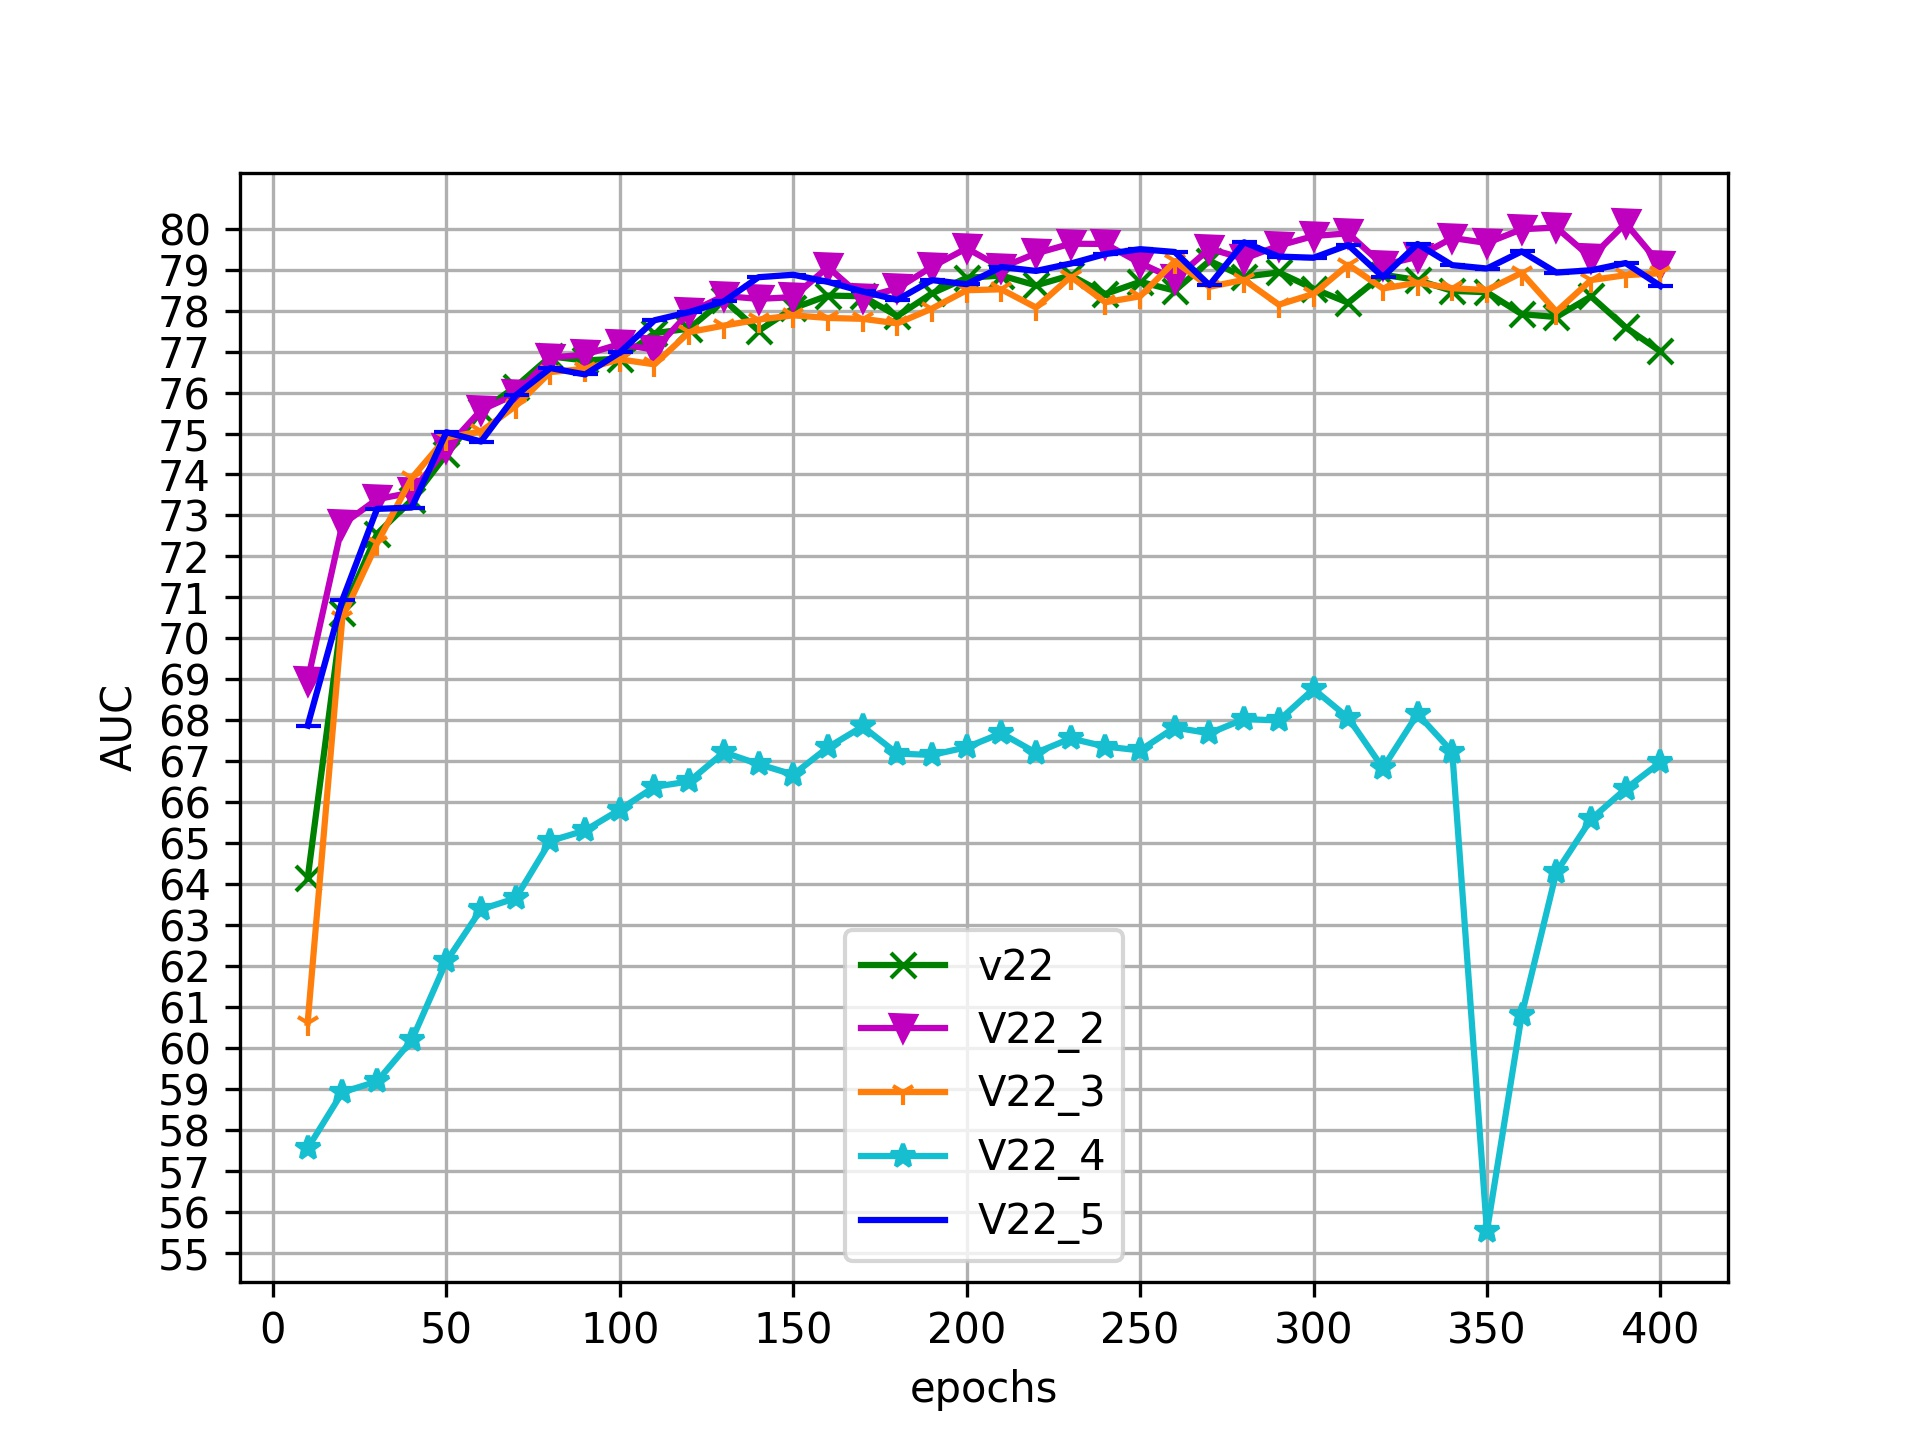
\includegraphics[trim=0 0 0 0, clip, width=1.\linewidth]{images/exp_1.jpg}
	\caption{Performance comparison, changing $NF$ the number of frames in input to the VST  (from 1 to 5).}
	\label{fig:num-frames-vst}
\end{figure}

\begin{figure}[t]
\centering
	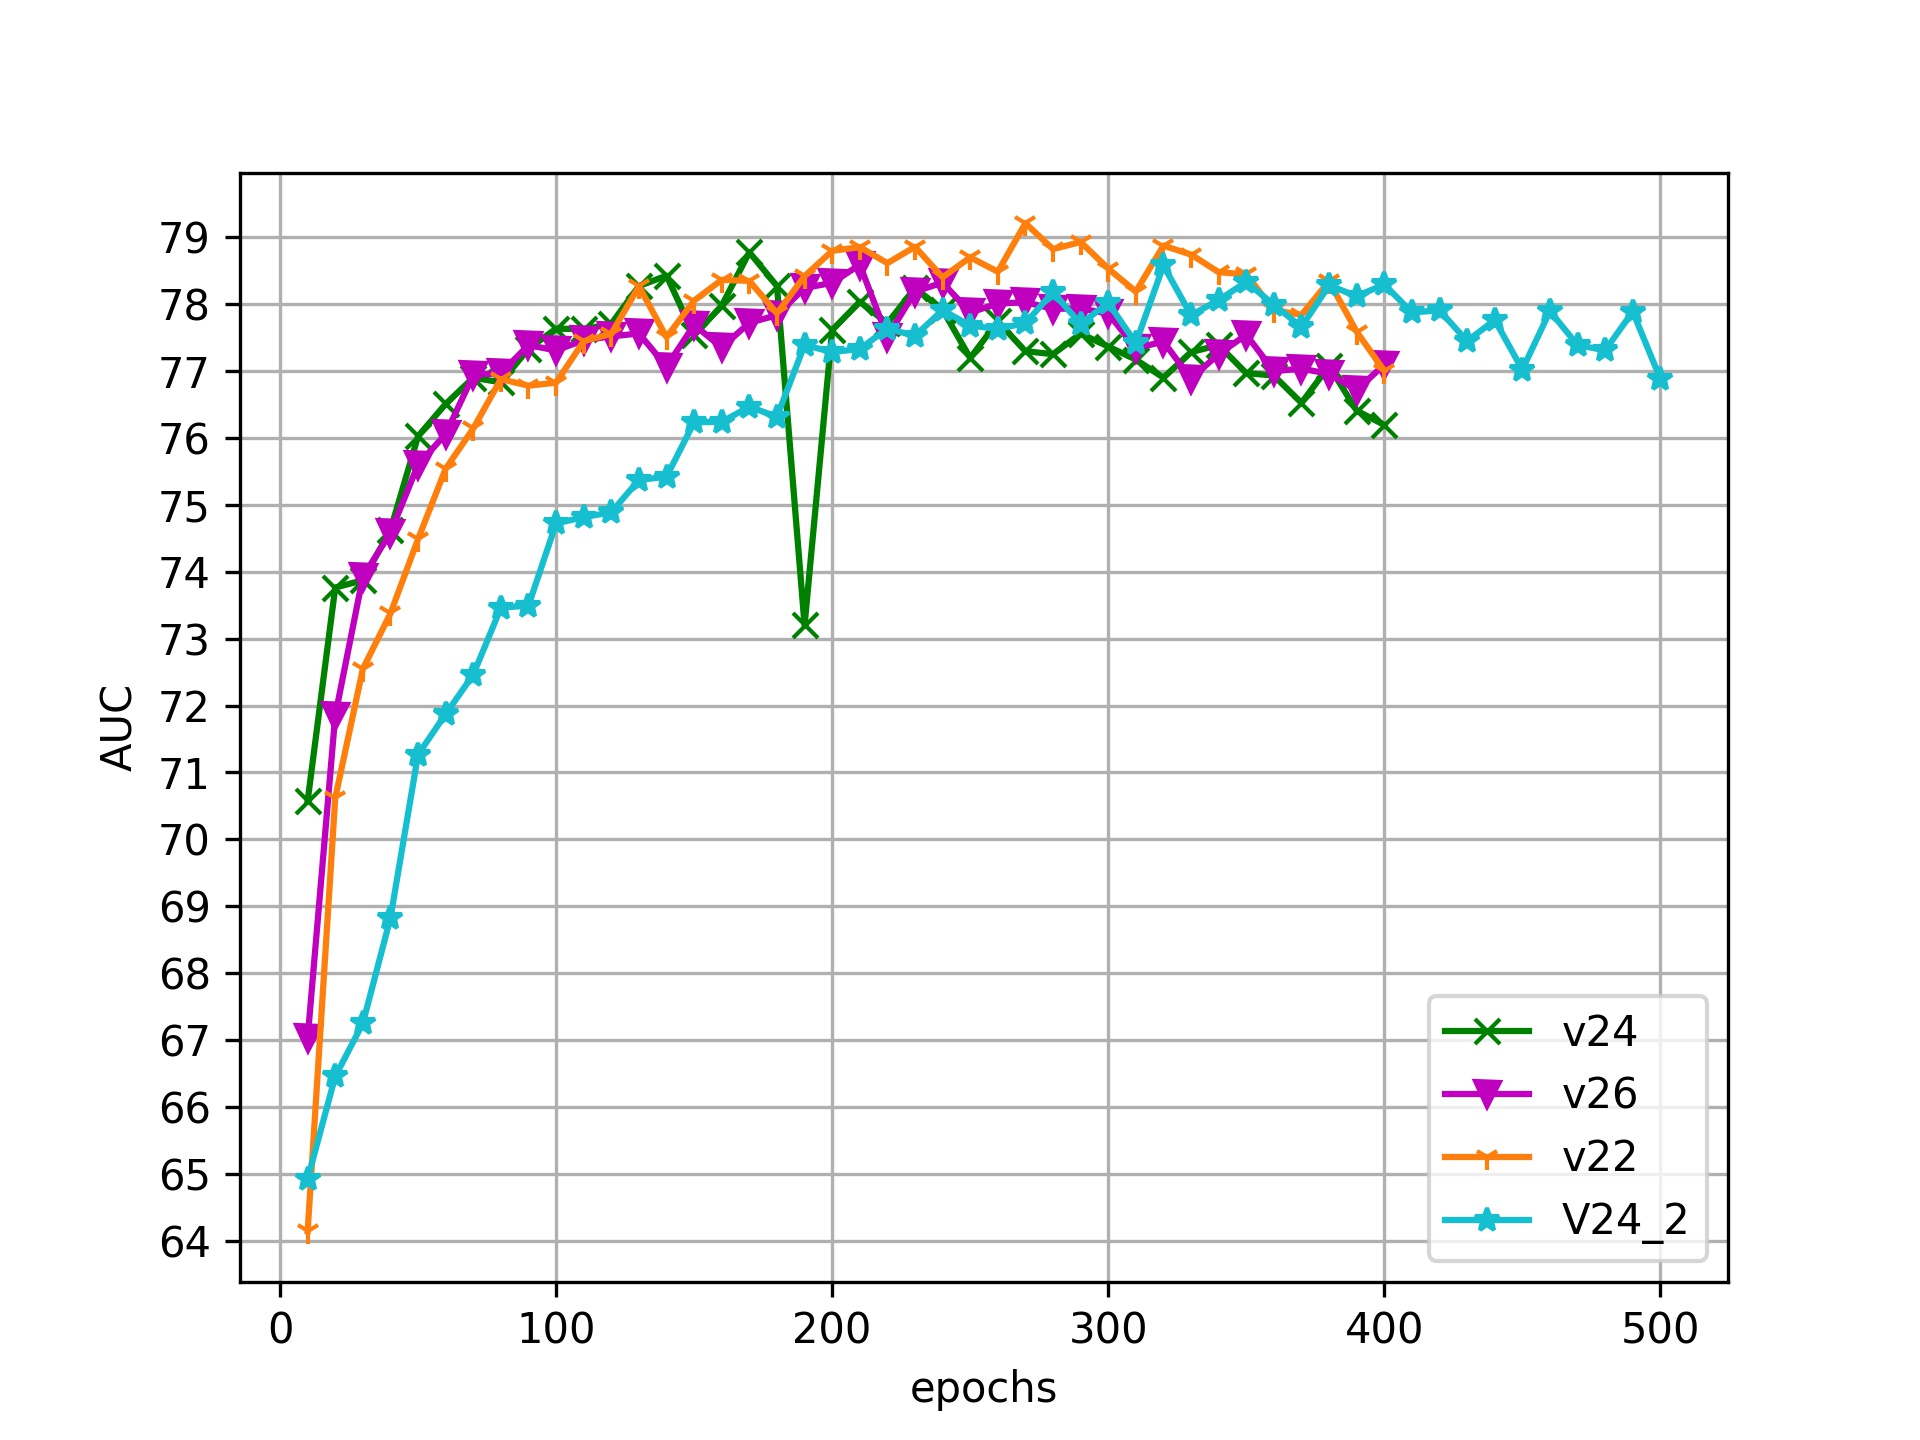
\includegraphics[trim=0 0 0 0, clip, width=1.\linewidth]{images/exp_2.jpg}
    % TODO aggiorna caption!
	\caption{Performance comparison, changing the number of LSTM cells (from 0 to 4) that form the long-term memory. "LSTM 2 cells" is the same as NF 3 of previous experiment in Fig.~\ref{fig:num-frames-vst}.}
	\label{fig:num-memory-cells}
\end{figure}

\begin{figure}[t]
\centering
	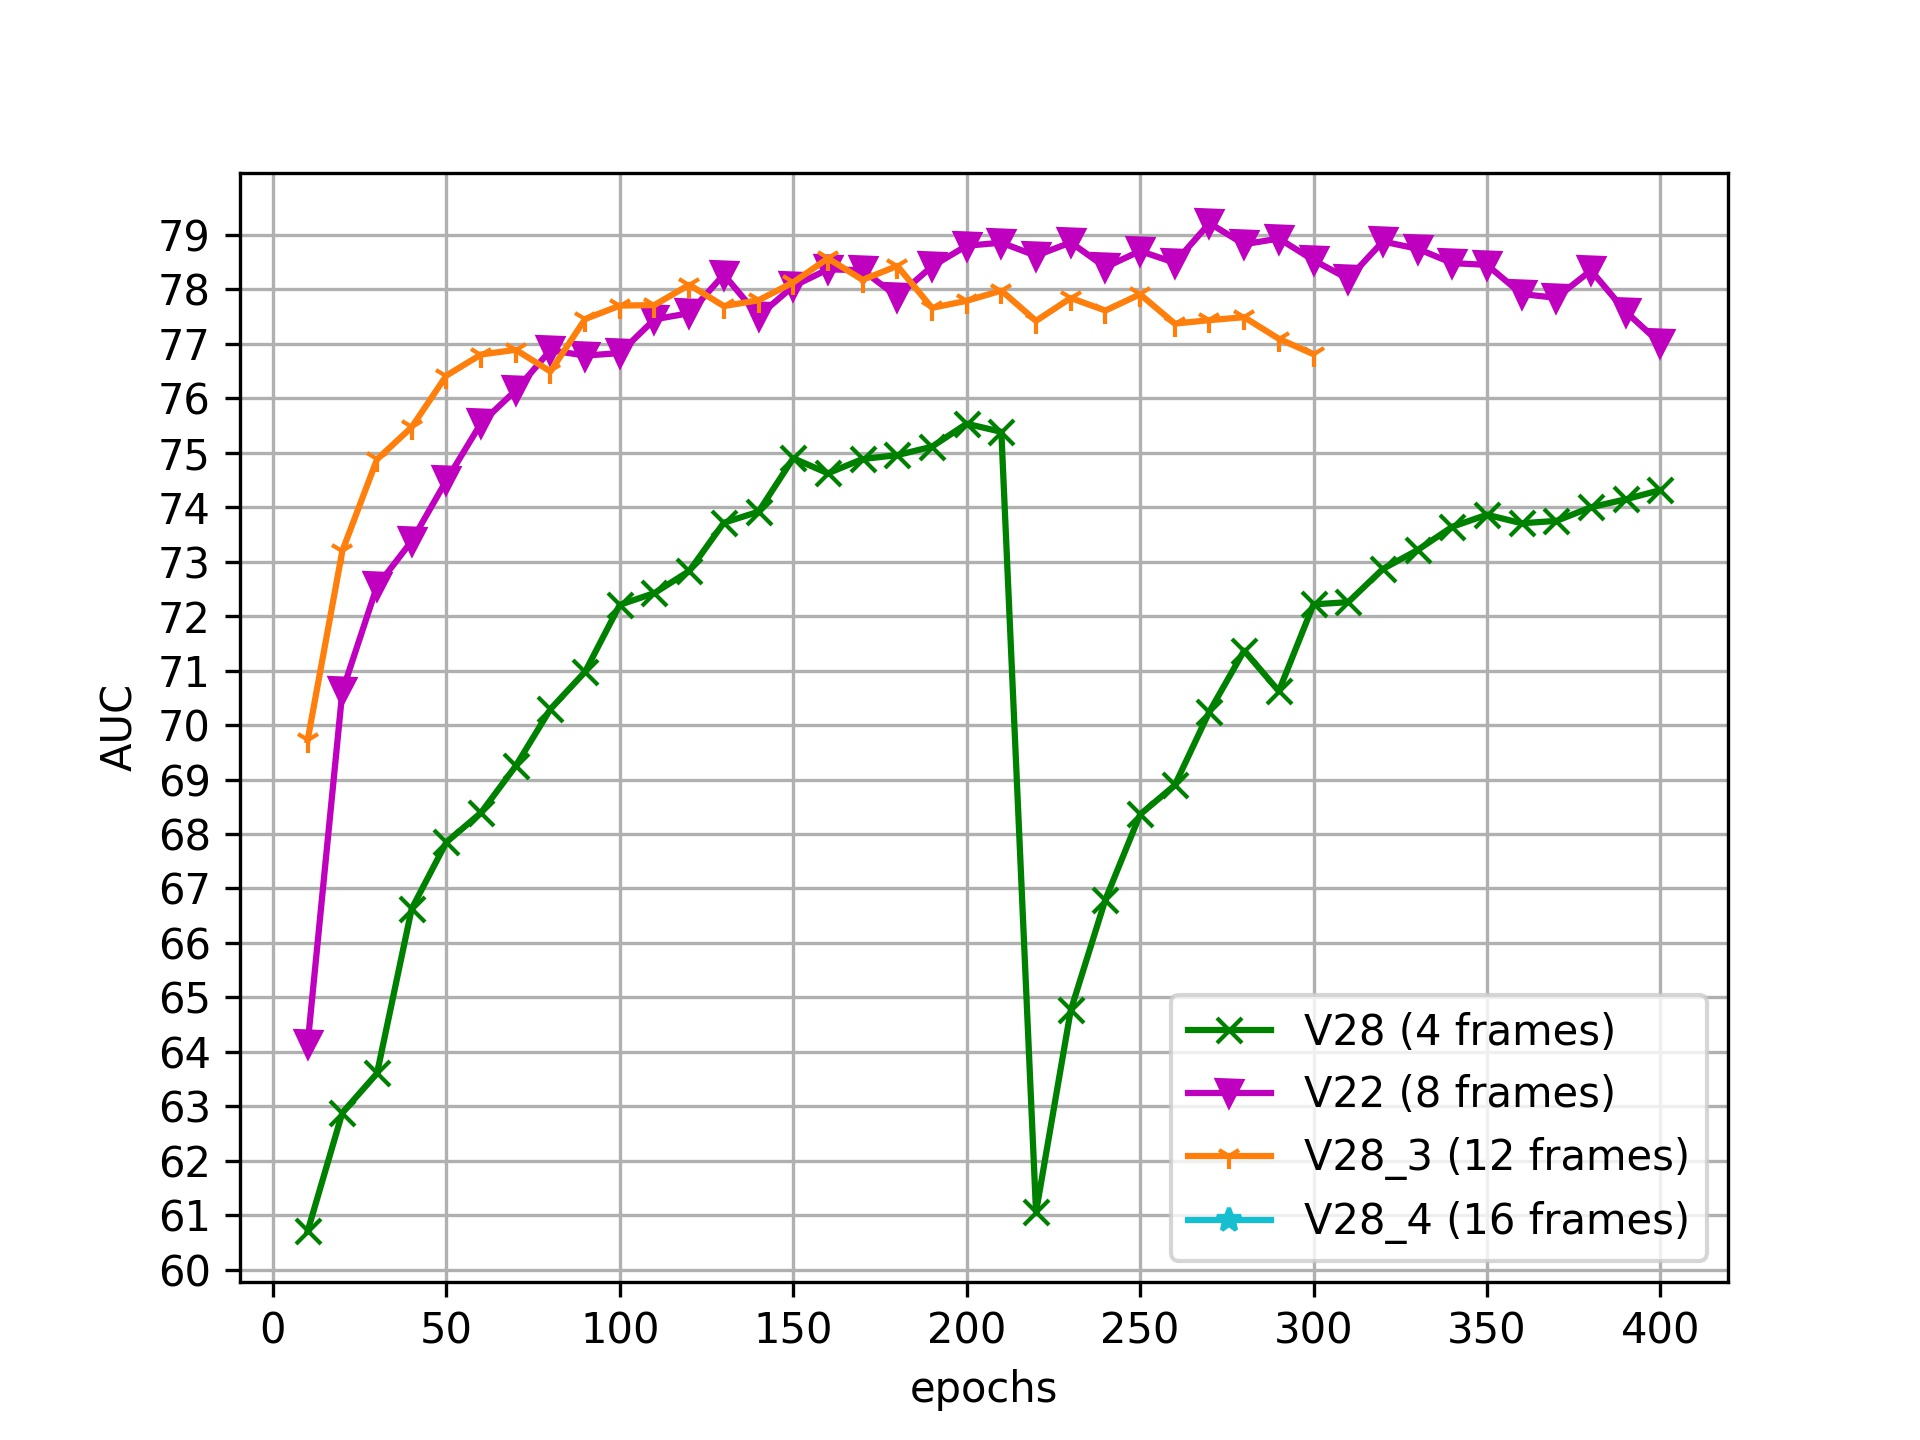
\includegraphics[trim=0 0 0 0, clip, width=1.\linewidth]{images/exp_3.jpg}
    % TODO aggiorna caption!
	\caption{Performance comparison, changing the video clip length (from 4 to 16). The "8 frames" configuration is the same as the NF 3 configuration of previous experiment in Fig.~\ref{fig:num-frames-vst}.}
	\label{fig:random-batch}
\end{figure}

\begin{table}[b]
	\footnotesize
	%\setlength{\tabcolsep}{1.2pt}
	\begin{center}
		\begin{tabular}{!r|^l|^l|^c|}
			\# & Method & Input & $AUC$ \\
			\hline\hline
	   	              1 & ConvAE \cite{hasan2016learning} & Gray & 64.3 \\
			        2 & ConvAE \cite{hasan2016learning} & Flow & 66.3 \\
                    3 & ConvLSTMAE \cite{chong2017abnormal} & Gray & 53.8 \\
                    4 & ConvLSTMAE \cite{chong2017abnormal} & Flow & 62.5 \\
                    5 & AnoPred \cite{liu2018future} & RGB & 67.5 \\
                    6 & AnoPred \cite{liu2018future} & Masked RGB & 64.8 \\
                    7 & FOL-Ensemble \cite{9712446} & RGB + Box + Flow + Ego & 73.0 \\
                    8 & STFE \cite{zhou_spatio-temporal_2022} & RGB + Flow & 79.3 \\
            \hline
                    % v22_2
\rowstyle{\bfseries}9 & Our (MOVAD) & RGB ($320\times240$) &  80.13 \\
                    % v30_3
%\rowstyle{\bfseries}9 & Our (MOVAD) & RGB ($320\times240$) &  XXX \\
                    % v30
\rowstyle{\bfseries}10 & Our (MOVAD) & RGB ($640\times480$) &  82.05 \\
\end{tabular}
	\end{center}
	\caption{Benchmarks of VAD (Video Anomaly Detection) methods on the DoTA dataset. \lnote{aggiungi risultati v30\_3, dato che $v30\_2 \ge v30$, e descrivi le caratteristiche}}
	\label{tab:sota-vad-auc}
\end{table}

% TODO visualizza anche la colonna OO e VO? (VO and OO columns are not shown because they do not contain anomalous traffic participants)
\begin{table*}[ht]
	\footnotesize
	\setlength{\tabcolsep}{3.7pt}
	\begin{center}
		\begin{tabular}{|!l||^c|^c|^c|^c|^c|^c|^c|^c|^c|^c|^c|^c|^c|^c|^c|^c|^c|^c|}
			Model & $ST$ & $AH$ & $LA$ & $OC$ & $TC$ & $VP$ & $VO$ & $OO$ & $UK$ & $ST*$ & $AH*$ & $LA*$ & $OC*$ & $TC*$ & $VP*$ & $VO*$ & $OO*$ & $UK*$ \\
			\hline\hline
                AnoPred \cite{liu2018future}          & 69.9 & 73.6 & 75.2 & 69.7 & 73.5 & 66.3 & N.D. & N.D. & N.D. & 70.9 & 62.6 & 60.1 & 65.6 & 65.4 & 64.9 & 64.2 & 57.8 & N.D. \\
                AnoPred \cite{liu2018future} + Mask   & 66.3 & 72.2 & 64.2 & 65.4 & 65.6 & 66.6 & N.D. & N.D. & N.D. & 72.9 & 63.7 & 60.6 & 66.9 & 65.7 & 64.0 & 58.8 & 59.9 & N.D. \\
                FOL-STD \cite{9712446}                & 67.3 & 77.4 & 71.1 & 68.6 & 69.2 & 65.1 & N.D. & N.D. & N.D. & 75.1 & 66.2 & 66.8 & 74.1 & 72.0 & 69.7 & 63.8 & 69.2 & N.D. \\
                FOL-Ensemble \cite{9712446}           & 73.3 & 81.2 & 74.0 & 73.4 & 75.1 & 70.1 & N.D. & N.D. & N.D. & \red{77.5} & 69.8 & 68.1 & \red{76.7} & 73.9 & 71.2 & 65.2 & 69.6 & N.D. \\
                % STFE gli manca la colonna VP*!
                % STFE ha dei risultati non molto chiari.
                STFE \cite{zhou_spatio-temporal_2022} & 75.2 & \red{84.5} & 72.1 & 77.3 & 72.8 & 71.9 & N.D. & N.D. & N.D. & \textbf{80.6} & 65.6 & \red{69.9} & 76.5 & 74.2 & N.D. & \red{75.6} & \red{70.5} & N.D. \\
                % v22_2 epoca 320
                \textbf{Our (MOVAD)}                  &  \red{85.6} & \red{84.5} & \red{81.4} & \red{82.8} & \red{84.9} & \textbf{85.8} & \textbf{79.1} & \textbf{87.4} & \textbf{76.2} & 75.1 & \red{69.9} & 68.4 & 76.6 & \red{75.8} & \red{71.8} & 74.1 & 70.2 & \red{69.4} \\
                % v30
                %\textbf{Our (MOVAD)} &  \textbf{86.7} & \textbf{86.7} & \textbf{84.1} & \textbf{83.2} & \textbf{86.1} & \textbf{81.9} & 73.2 & \textbf{70.2} & \textbf{74.5} & \textbf{80.0} & \textbf{77.7} & \textbf{75.5} & \textbf{80.1} & \textbf{78.0}  \\
                % v30_2 (epoca 450)
                \textbf{Our (MOVAD) **}                  &  \textbf{87.2} & \textbf{86.6} & \textbf{85.0} & \textbf{83.8} & \textbf{86.2} & \red{79.1} & \red{77.9} & \red{87.1} & \red{74.1} & 72.8 & \textbf{73.1} & \textbf{75.7} & \textbf{82.2} & \textbf{79.0} & \textbf{74.7} & \textbf{80.3} & \textbf{77.8} & \textbf{72.1} \\
        \hline
\end{tabular}
	\end{center}
	\caption{Detection accuracy for each individual accident category (AUC) on VAD task. "*" indicates non-ego anomaly categories. "**" indicates input video resolution is $640\times480$ instead of $320\times240$. N.D. (Not Defined): means no value is available on paper that describes the corresponding model. Bold and red values are respectively the best and second-best results.\lnote{aggiungi anche v22\_2 o 30\_3}}
	\label{tab:sota-vad-auc-per-class}
\end{table*}

\noindent\textbf{Dataset}.
We perform our tests on the DoTa dataset \cite{9712446}.
It contains 4677 videos taken from YouTube channels, with a resolution of $1280 \times 720$, annotated with information about the start and end of the anomaly, the category (10 in total) and the bounding boxes of the objects or persons involved.
The videos were recorded in different countries and with different light and weather conditions.
We use the original dataset split, in approximately $70\%$ training and $30\%$ validation.
Our benchmarks are related to the Task~1~\cite{9712446}, the (frame-level) Video Anomaly Detection.
Our model training and evaluation takes place in the online scenario, that is the most realistic, and most interesting condition from our point of view.

\noindent\textbf{Evaluation Metrics}.
To evaluate the performance of the models, we use the well-known Area Under Curve (AUC) metric at frame-level.
This metric evaluate how well the model temporally locate the anomaly in the videos. 

\noindent\textbf{Implementation details.}
%The results of the models, with which we compare, are taken from the respective papers.
We perform the training on a single machine with a A100 GPU.
We use the Stochastic Gradient Descent (SGD) optimization algorithm with a learning rate of 0.0001, a momentum of 0.9, video clip length 8 and batch size 8.
We use SGD instead of Adam because in our experiments the latter led the training to be unstable, resulting in the model diverging after a few epochs.

\noindent\textbf{Training details.}
Because the videos contain a non-uniform number of frames, we fixed the number of frames for each video taken into account (video clip length) in order to be able to train the model with a batch size larger than one.
At each iteration, we randomly choose the starting frame for each video, adjusting the ground-truth accordingly. This makes the training as diverse as possible and reduce the effect of overfitting.
Unless otherwise specified, the input video shape is $320 \times 240$, video clip length is 8, LSTM cell number is 2, input number of frames of VST (NF) is 3 and the classification head is initialized using a uniform distribution for Linear weights, with a (semi) orthogonal matrix for LSTM modules and bias parameters set to zero, the VST weights are initialized with a model pretrained on Something-Something v2 \cite{goyal2017something}.

\subsection{Ablation study}
\tnote{Ho visto che qui alla fine ci compariamo con lo stato dell'arte, farei due sezioni separate (tipo Ablation ed Experimental Results) oppure cambierei nome a questa sezione che dite? :)}
% class weight loss
% 2xsoftmax vs 1x
% learning rate differences (sto finendo l’esperimento con multipli lr)

\noindent\textbf{Short-term memory module.}

% v22: numero di frames in input
In this experiment, we empirically show the effects of the input frames to the Short-term memory module, varying the number of frames processed by the VST at each step.
The results are displayed in the Fig.~\ref{fig:num-frames-vst}.
As we expected, taking into account only the current frame is the worst situation, making the training more unstable.
This is reasonable as the short-term memory module processes and embeds only the current frame, without any knowledge of the near past, leading the long-term memory module to overfit data since consecutive frames are very similar. \vnote{confermare con esperimento NF=1 e no LSTM}
Increasing the number of frames processed at each step has a much more limited effect. Indeed, with 5 frames the effect already becomes counterproductive since the increased amount of information processed is not justified by a gain in performance.
The highest AUC is obtained with 4 frames.

% (no) v23: rand frame order (v17) vs normal
% v29_2, v29, v22: training from scratch vs pretrained (imagenet vs smth2smthv2)

\noindent\textbf{Long-term memory module.}
% posizione dell'lstm senza / prima / dopo / prim + dopo / gru
% v24_4: senza lstm
% v24, v22, v24_2: 1/2/3 # celle lstm
% v26, v26_2, v26_3: 1/2/3 # celle gru
% (no) v27, v27_2: pre + post lstm (1 cell) + saliency (?), pre + post lstm (1 cell)
In this experiment, we evaluate the long-term memory effect on the classification capability.
In Fig.~\ref{fig:num-memory-cells}, we compare the network with and without the LSTM long-term memory.
For the long-term memory, we test the LSTM and the GRU \cite{chung2014empirical} modules, with a number of cells varying from 1 to 4.
To make the Figure easier to read, the GRU results are not shown, but the trend does not differ much from the LSTM module. 
The effect introduced by the memory cells is evident.
Having no cell makes training slower in saturating performance and it reaches the lowest AUC value.
With one cell the performances saturate very quickly, with a slow degradation during the rest of the epochs.
By increasing the number of cells, the achievement of the maximum peak is slowed down over time, but in absolute value it is higher, converging towards similar values.
The maximum AUC is reached by 2 LSTM cells around epoch 270.
\lnote{v30\_2: check se aggiungere pezzo relativo a: alla fine la migliore è con 3 celle perchè il picco lo raggiunge verso 400 epoche quando interessa maggiormente a noi}

%\noindent\textbf{Saliency module.}
% v25, v22: con/senza/versione ridotta della saliency
%In this experiment, we evaluate the effect of the saliency branch.

\noindent\textbf{Video clip length.}
% v22, v28: random_batch 4/8/12/16/20/24: describi la modalità di addestramento -> per usare un batch size > 1 si è scelto di selezionare un numero max di frame da elaborare a ogni iterazione. per aggiungere diversità al training, il punto di inizio per ogni video viene scelto in modo casuale a ogni iterazione, adattando di conseguenza il ground-truth
As mentioned in training details subsection, at each iteration and separately for each video, a random starting point is selected and a fixed number of frames (video clip length) is used to train the network.
In Figure \ref{fig:random-batch}, we evaluate the effect of the size of the video clip length.
The worse and most unstable training is obtained with 4 frames, probably because they are too few to exploit the long-term memory effect of LSTM cells.
Increasing the clip length permits to saturate performance quicker, but a value too high (like 12 or 16) tends to produce a lower AUC overall.
In fact, the highest AUC value is obtained using 8 frames as video clip length, which represents a good balance between enlarging clip size and exploiting LSTM cells while, at the same time, avoid overfitting due to consecutive frames being too similar to each other.

\noindent\textbf{MOVAD model}
% input shape
% versione finale vs resto del mondo su dota, and: 
%   - Phantom: https://paperswithcode.com/paper/approaches-toward-physical-and-general-video
%   - ShanghaiTech: https://paperswithcode.com/sota/anomaly-detection-on-shanghaitech
%   - CUHK Avenue: https://paperswithcode.com/sota/anomaly-detection-on-chuk-avenue
%   - UCSD Ped2: https://paperswithcode.com/sota/abnormal-event-detection-in-video-on-ucsd
Finally, in Table \ref{tab:sota-vad-auc} we compare our model performance with state of the art models using in input video shape of $320\times240$ and $640\times480$, with video clip length of 8, 3 LSTM cells and $NF=3$.
Table \ref{tab:sota-vad-auc-per-class} shows results per class (see \cite{9712446} for acronyms meaning).
Our MOVAD architecture surpasses the state-of-the-art model by $+2.75\%$ AUC, reaching the highest value of $82.05\%$.
%VB: Potrebbe servire come confronto per il numero parametri e flops
%sembra non riesca a calcolare i flops della rnn però
%| module                    | #parameters or shape   | #flops     |
%|:--------------------------|:-----------------------|:-----------|
%| model                     | 0.144G                 | 0.208T     |
%|  rnn                      |  16.794M               |  0         |
%|   rnn.weight_ih_l0        |   (4096, 1024)         |            |
%|   rnn.weight_hh_l0        |   (4096, 1024)         |            |
%|   rnn.bias_ih_l0          |   (4096,)              |            |
%|   rnn.bias_hh_l0          |   (4096,)              |            |
%|   rnn.weight_ih_l1        |   (4096, 1024)         |            |
%|   rnn.weight_hh_l1        |   (4096, 1024)         |            |
%|   rnn.bias_ih_l1          |   (4096,)              |            |
%|   rnn.bias_hh_l1          |   (4096,)              |            |
%|  rnn_bn                   |  2.048K                |  5.12K     |
%|   rnn_bn.weight           |   (1024,)              |            |
%|   rnn_bn.bias             |   (1024,)              |            |
%|  lin1                     |  37.75M                |  37.749M   |
%|   lin1.weight             |   (1024, 36864)        |            |
%|   lin1.bias               |   (1024,)              |            |
%|  lin2                     |  1.05M                 |  1.049M    |
%|   lin2.weight             |   (1024, 1024)         |            |
%|   lin2.bias               |   (1024,)              |            |
%|  lin3                     |  2.05K                 |  2.048K    |
%|   lin3.weight             |   (2, 1024)            |            |
%|   lin3.bias               |   (2,)                 |            |
%|  bn                       |  73.728K               |  0.184M    |
%|   bn.weight               |   (36864,)             |            |
%|   bn.bias                 |   (36864,)             |            |
%|  model                    |  88.656M               |  0.208T    |
%|   model.patch_embed       |   12.672K              |   0.496G   |
%|    model.patch_embed.proj |    12.416K             |    0.472G  |
%|    model.patch_embed.norm |    0.256K              |    24.576M |
%|   model.layers            |   88.641M              |   0.208T   |
%|    model.layers.0         |    0.571M              |    18.801G |
%|    model.layers.1         |    2.19M               |    17.997G |
%|    model.layers.2         |    60.353M             |    0.153T  |
%|    model.layers.3.blocks  |    25.528M             |    17.831G |
%|   model.norm              |   2.048K               |   3.072M   |
%|    model.norm.weight      |    (1024,)             |            |
%|    model.norm.bias        |    (1024,)             |            |